\documentclass[fleqn, a4paper, 10pt, oneside]{amsart}
\usepackage{exsheets}
\usepackage{amsmath, amssymb, amsthm} %standard AMS packages
\usepackage{marginnote} %marginnotes
\usepackage{gensymb} %miscellaneous symbols
\usepackage{commath} %differential symbols
\usepackage{xcolor} %colours
\usepackage{cancel} %cancelling terms
\usepackage[free-standing-units, space-before-unit]{siunitx} %formatting units
\usepackage{tikz, pgfplots} %diagrams
	\usetikzlibrary{calc, hobby, patterns, intersections, decorations.markings}
\usepackage{graphicx} %inserting graphics
\usepackage{hyperref} %hyperlinks
\usepackage{datetime} %date and time
\usepackage{enumerate,enumitem} %numbered lists
\usepackage{float} %inserting floats
\usepackage{circuitikz}[american voltages, american currents] %circuit diagrams
\usepackage{booktabs}
\usepackage{csvsimple}
\usepackage{todonotes}

\newcommand\numberthis{\addtocounter{equation}{1}\tag{\theequation}} %adds numbers to specific equations in non-numbered list of equations

\theoremstyle{definition}
\newtheorem{example}{Example}
\newtheorem{definition}{Definition}

\theoremstyle{theorem}
\newtheorem{theorem}{Theorem}

\makeatletter
\@addtoreset{section}{part} %resets section numbers in new part
\makeatother

\SetupExSheets{solution/print = true}

%opening
\title
[
	Electronic Devices : Assignment 3
]
{
	Electronic Devices\\
	Assignment 3
}
\author
{
	Aakash Jog\\
	ID : 989323563
}
\date{\formatdate{31}{3}{2016}}

\begin{document}

\maketitle
%\setlength{\mathindent}{0pt}

\begin{question}
	A silicon PN junction maintained at $T = 300 \kelvin$ has doping profile
	\begin{align*}
		N_D - N_A &= N_0 \left( 1 - e^{-\alpha x} \right)
	\end{align*}
	where $N_0$ and $\alpha$ are constant.
	\begin{enumerate}
		\item Sketch the charge density as a function of $x$.
		\item Establish an expression for the field distribution as a function of position $x$.
	\end{enumerate}
\end{question}

\begin{solution}
	\begin{enumerate}[leftmargin=*]
		\item
			\begin{align*}
				\rho(x) &= q (N_D - N_A)\\
				&= q N_0 \left( 1 - e^{-\alpha x} \right)
			\end{align*}
		\item
			\begin{align*}
				\mathcal{E}(x) &= \int \frac{\rho(x)}{\varepsilon \varepsilon_0} \dif x\\
				&= \frac{q N_0}{\varepsilon \varepsilon_0} \int \left( 1 - e^{-\alpha x} \right) \dif x\\
				&= \frac{q N_0}{\varepsilon \varepsilon_0} \left( x + \frac{e^{-\alpha x}}{\alpha} + c \right)
			\end{align*}
			At the boundaries of the depletion region,
			\begin{align*}
				\mathcal{E}(-x_p) &= 0\\
				\mathcal{E}(x_n) &= 0
			\end{align*}
			Therefore,
			\begin{align*}
				0 &= \frac{q N_0}{\varepsilon \varepsilon_0} \left( -x_p + \frac{e^{\alpha x_p}}{\alpha} + c \right)\\
				\therefore x &= x_p - \frac{e^{\alpha x_p}}{\alpha}
			\end{align*}
			Therefore,
			\begin{align*}
				\mathcal{E}(x) &= \frac{q N_0}{\varepsilon \varepsilon_0} \left( x + \frac{e^{-\alpha x}}{\alpha} + x_p - \frac{e^{\alpha x_p}}{\alpha} \right)
			\end{align*}
	\end{enumerate}
\end{solution}

\begin{question}
	Consider a silicon PN step junction with
	\begin{align*}
		N_A &= 5 \times 10^{15} \si{\per\centi\metre\cubed}\\
		N_D &= 10^{14} \si{\per\centi\metre\cubed}
	\end{align*}
	maintained at $T = 300 \kelvin$.
	\begin{enumerate}
		\item
			Calculate $V_{\text{BI}}$, $x_n$, and $x_p$ at zero applied bias.
		\item
			To increase $x_n$ beyond the equilibrium value found above, what polarity of voltage should be applied?
			Sketch the PN junction, showing the applied bias, specifically which polarity is applied to each side.
		\item
			Calculate the required bias for $x_n = 30 \si{\micro\metre}$.
		\item
			Sketch the energy band diagram for the above bias.
		\item
			Calculate $x_n$ for the magnitude of applied voltage calculated above divided by $200$ with the opposite polarity.
		\item
			Sketch the energy band diagram for the above bias.
		\item
			On the same plot above, sketch the electric field across the device for all three cases: $V = 0$, $V > 0$, and $V < 0$.
			On the plot, indicate the areas under the electric field curve that correspond to $V_{\text{BI}}$, $V_{\text{forward}}$, and $V_{\text{reverse}}$.
	\end{enumerate}
\end{question}

\begin{solution}
	\begin{enumerate}[leftmargin=*]
		\item
			As the junction is a step junction,
			\begin{align*}
				V_{BI} &= \frac{k T}{q} \ln\left( \frac{N_A N_D}{{n_i}^2} \right)\\
				&= \frac{k T}{q} \ln\left( \frac{5 \times 10^{29}}{10^{20}} \right)\\
				&= \frac{k T}{q} \ln\left( 5 \times 10^9 \right)\\
				&= (0.0257) (22.33270375)\\
				&= 0.5739504864 \volt
			\end{align*}
			Therefore,
			\begin{align*}
				W &= \sqrt{\frac{2 \varepsilon \varepsilon_0 V_{\text{BI}}}{q} \left( \frac{N_A + N_D}{N_A N_D} \right)}\\
				&= \sqrt{\frac{(2) (11.8) \left( 8.85 \times 10^{-14} \right) (0.574)}{q} \left( \frac{51 \times 10^{14}}{5 \times 10^{29}} \right)}\\
				&= 2.76455 \times 10^{-4} \si{\centi\metre}\\
				&= 2.76455 \si{\micro\metre}
			\end{align*}
			Therefore,
			\begin{align*}
				x_p &= W \frac{N_D}{N_A + N_D}\\
				&= 2.76455 \frac{10^{14}}{51 \times 10^{14}}\\
				&= 5.42068 \times 10^{-6} \si{\centi\metre}\\
				&= 0.0542068 \si{\micro\metre}\\
				x_n &= W \frac{N_A}{N_A + N_D}\\
				&= 2.76455 \frac{50 \times 10^{14}}{51 \times 10^{14}}\\
				&= 2.71034 \times 10^{-4} \si{\centi\metre}\\
				&= 2.71034 \si{\micro\metre}
			\end{align*}
		\item
			The width of the depletion region increases if the PN junction is in reverse bias.
			Therefore, the voltage should connected as shown.
			\begin{figure}[H]
				\centering
				\begin{tikzpicture}
					\def\l{2};
					\def\h{1};
					\def\xP{0.25};
					\def\xN{0.5};

					\begin{scope}
						\draw (-\l,-\h/2) rectangle (0,\h/2);
						\draw (0,-\h/2) rectangle (\l,\h/2);
					\end{scope}
					
					\begin{scope}
						\draw (\l,0) -| (2*\l,-2*\h);
						\draw (-\l,0) -| (-2*\l,-2*\h);
						\draw (-2*\l,-2*\h) to [battery1 = $V_a$] (2*\l,-2*\h);
					\end{scope}

					\begin{scope}
						\node at (\l/2,0) {N};
						\node at (-\l/2,0) {P};
					\end{scope}
				\end{tikzpicture}
			\end{figure}
		\item
			\begin{align*}
				\frac{x_p}{x_n} &= \frac{N_D}{N_A}\\
				&= \frac{10^{14}}{5 \times 10^{15}}\\
				&= \frac{1}{50}\\
				&= 0.02\\
				\therefore x_p &= 0.02 x_n
			\end{align*}
			Therefore,
			\begin{align*}
				W &= x_p + x_n\\
				&= 1.02 x_n
			\end{align*}
			Therefore, for $x_n = 30 \si{\micro\metre}$,
			\begin{align*}
				W &= (1.02) (30)\\
				&= 30.6 \si{\micro\metre}
			\end{align*}
			Therefore,
			\begin{align*}
				W &= \sqrt{\frac{2 \varepsilon \varepsilon_0 (V_{\text{BI}} + V_a)}{q} \left( \frac{N_A + N_D}{N_A N_D} \right)}\\
				30.6 &= \sqrt{\frac{(2) (11.8) \left( 8.85 \times 10^{-14} \right) (0.574 + V_a)}{q} \left( \frac{51 \times 10^{14}}{5 \times 10^{29}} \right)}\\
			\end{align*}
			Therefore, solving,
			\begin{align*}
				V_a &= -0.566968 \volt
			\end{align*}
		\item
			~\\
			\begin{figure}[H]
				\centering
				\begin{tikzpicture}[scale = 1.5]
					\def\eConductionP{3};
					\def\eConductionN{2};
					\def\eIntrinsicP{2};
					\def\eIntrinsicN{1};
					\def\eValenceP{1};
					\def\eValenceN{0};
					\def\eFermiP{1.75};
					\def\eFermiN{1.25};
					\def\l{3};
					\def\W{1};
			
					\begin{scope}
						\draw (-\l,\eConductionP) node [left] {$E_C$} -- (-\W/2,\eConductionP);
						\draw [dashed] (-\l,\eIntrinsicP) node [left] {$E_i$} -- (-\W/2,\eIntrinsicP);
						\draw (-\l,\eValenceP) node [left] {$E_V$} -- (-\W/2,\eValenceP);
					\end{scope}
			
					\begin{scope}
						\draw (-\W/2,\eConductionP) to [out = 0, in = 180] (\W/2,\eConductionN);
						\draw [dashed] (-\W/2,\eIntrinsicP) to [out = 0, in = 180] (\W/2,\eIntrinsicN);
						\draw (-\W/2,\eValenceP) to [out = 0, in = 180] (\W/2,\eValenceN);
					\end{scope}
			
					\begin{scope}
						\draw (\W/2,\eConductionN) -- (\l,\eConductionN) node [right] {$E_C$};
						\draw [dashed] (\W/2,\eIntrinsicN) -- (\l,\eIntrinsicN) node [right] {$E_i$};
						\draw (\W/2,\eValenceN) -- (\l,\eValenceN) node [right] {$E_V$};
					\end{scope}
			
					\begin{scope}
						\draw (-\l,\eFermiP) node [left] {$E_F$} -- (-\W/2,\eFermiP);
						\draw (\W/2,\eFermiN) -- (\l,\eFermiN) node [right] {$E_F$};
					\end{scope}
			
					\begin{scope}[dashed]
						\draw (-\W/2,\eConductionP + 1) -- (-\W/2,\eValenceN - 1);
						\draw (\W/2,\eConductionP + 1) -- (\W/2,\eValenceN - 1);
						\node [above] at (-\l/2 - \W/4,\eConductionP + 1) {P-type};
						\node [above] at (\l/2 + \W/4,\eConductionP + 1) {N-type};
						\node [above] at (0,\eConductionP + 1) {depletion region};
					\end{scope}
				\end{tikzpicture}
			\end{figure}
		\item
			\begin{align*}
				V_a &= -\frac{0.566968}{200}\\
				&= 0.00283484
			\end{align*}
			Therefore,
			\begin{align*}
				W &= \sqrt{\frac{2 \varepsilon \varepsilon_0 (V_{\text{BI}} + V_a)}{q} \left( \frac{N_A + N_D}{N_A N_D} \right)}\\
				&= 0.000277136 \si{\centi\metre}\\
				&= 2.77136 \si{\micro\metre}
			\end{align*}
			Therefore,
			\begin{align*}
				x_n &= W \frac{N_A}{N_A + N_D}\\
				&= 2.71702 \si{\micro\metre}
			\end{align*}
		\item
			~\\
			\begin{figure}[H]
				\centering
				\begin{tikzpicture}[scale = 1.5]
					\def\eConductionP{3};
					\def\eConductionN{2};
					\def\eIntrinsicP{2};
					\def\eIntrinsicN{1};
					\def\eValenceP{1};
					\def\eValenceN{0};
					\def\eFermiP{1.25};
					\def\eFermiN{1.75};
					\def\l{3};
					\def\W{1};
			
					\begin{scope}
						\draw (-\l,\eConductionP) node [left] {$E_C$} -- (-\W/2,\eConductionP);
						\draw [dashed] (-\l,\eIntrinsicP) node [left] {$E_i$} -- (-\W/2,\eIntrinsicP);
						\draw (-\l,\eValenceP) node [left] {$E_V$} -- (-\W/2,\eValenceP);
					\end{scope}
			
					\begin{scope}
						\draw (-\W/2,\eConductionP) to [out = 0, in = 180] (\W/2,\eConductionN);
						\draw [dashed] (-\W/2,\eIntrinsicP) to [out = 0, in = 180] (\W/2,\eIntrinsicN);
						\draw (-\W/2,\eValenceP) to [out = 0, in = 180] (\W/2,\eValenceN);
					\end{scope}
			
					\begin{scope}
						\draw (\W/2,\eConductionN) -- (\l,\eConductionN) node [right] {$E_C$};
						\draw [dashed] (\W/2,\eIntrinsicN) -- (\l,\eIntrinsicN) node [right] {$E_i$};
						\draw (\W/2,\eValenceN) -- (\l,\eValenceN) node [right] {$E_V$};
					\end{scope}
			
					\begin{scope}
						\draw (-\l,\eFermiP) node [left] {$E_F$} -- (-\W/2,\eFermiP);
						\draw (\W/2,\eFermiN) -- (\l,\eFermiN) node [right] {$E_F$};
					\end{scope}
			
					\begin{scope}[dashed]
						\draw (-\W/2,\eConductionP + 1) -- (-\W/2,\eValenceN - 1);
						\draw (\W/2,\eConductionP + 1) -- (\W/2,\eValenceN - 1);
						\node [above] at (-\l/2 - \W/4,\eConductionP + 1) {P-type};
						\node [above] at (\l/2 + \W/4,\eConductionP + 1) {N-type};
						\node [above] at (0,\eConductionP + 1) {depletion region};
					\end{scope}
				\end{tikzpicture}
			\end{figure}
		\item
			The electric fields corresponding to the biases are as shown.
			The areas under the curves represent the corresponding voltages.
			~\\
			\begin{figure}[H]
				\centering
				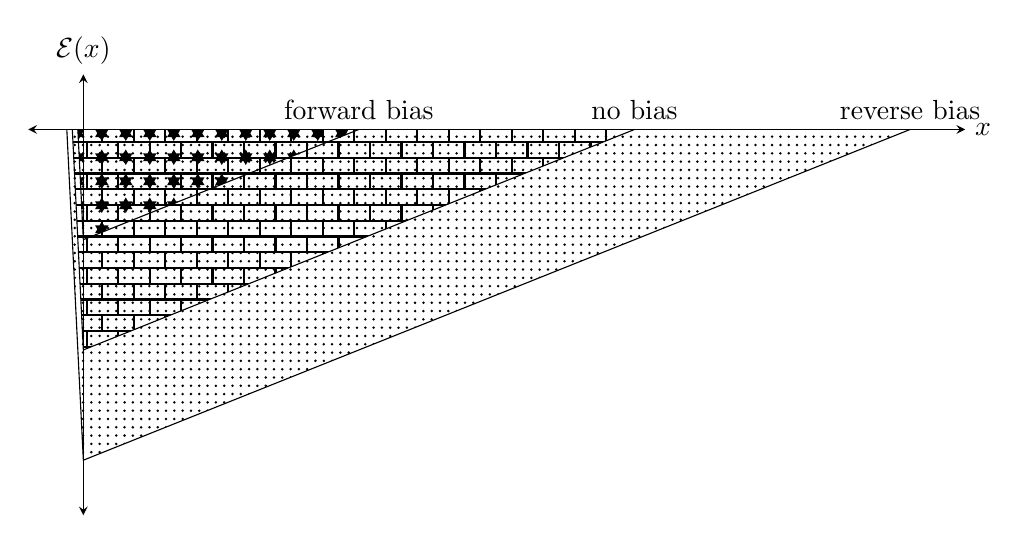
\begin{tikzpicture}[scale = 0.7]
					\def\xMIN{-1};
					\def\xMAX{16};
					\def\yMIN{-7};
					\def\yMAX{1};

					\def\xPF{0.1};
					\def\xNF{5};
					\def\EMaxF{2};

					\def\xPEq{0.2};
					\def\xNEq{10};
					\def\EMaxEq{4};

					\def\xPR{0.3};
					\def\xNR{15};
					\def\EMaxR{6};

					\begin{scope}[stealth-stealth]
						\draw (\xMIN,0) -- (\xMAX,0) node [right] {$x$};
						\draw (0,\yMIN) -- (0,\yMAX) node [above] {$\mathcal{E}(x)$};
					\end{scope}

					\begin{scope}
						\draw [pattern = bricks] (-\xPEq,0) -- (0,-\EMaxEq)-- (\xNEq,0) node [above] {no bias};
						\draw [pattern = sixpointed stars] (-\xPF,0) -- (0,-\EMaxF)-- (\xNF,0) node [above] {forward bias};
						\draw [pattern = dots] (-\xPR,0) -- (0,-\EMaxR)-- (\xNR,0) node [above] {reverse bias};
					\end{scope}
				\end{tikzpicture}
			\end{figure}
	\end{enumerate}
\end{solution}

\end{document}
